\section{Working with branches}

\begin{frame}

\frametitle{Branches in git}
	
\begin{itemize}
	\item Branches are used for isolated experimenting (short-lived branches), and isolated feature development (long-lived branches)
	\item Branching often is encouraged
	\item Git is specifically designed for efficient work with branches
	\item A branch is \textbf{simply a pointer to a commit}
	\item The default branch name is \alert{master}
\end{itemize}	

\begin{block}{When do I need a branch?}
	\begin{itemize}
	\item When you are beginning to work on a new feature
	\item When you want to make experimental commits
	\item When you want to single out a change (can be several commits) for making a pull request
	\item Whenever you feel like it!
	\end{itemize}
\end{block}

\end{frame}

% -----------------------------------------------------------------------------

\begin{frame}[fragile]
	
\frametitle{Creating a branch}
	
Creating a branch:
\begin{minted}{console}
> git branch <branch name>
\end{minted}

Switching to a branch:
\begin{minted}{console}
> git checkout <branch name>
\end{minted}

Or, in one command:
\begin{minted}{console}
> git checkout -b <branch name>
\end{minted}
	
Listing local branches:
\begin{minted}{console}
> git branch -v
\end{minted}	

\begin{block}{Two uses of checkout}
	\begin{itemize}
	\item Notice that we have already used \texttt{checkout} for checking out an earlier version of a file. This does not the affect the head commit in any way.
	\item The \texttt{checkout} command is also used for switching to another branch, which of course changes the head commit (and the files in the working tree)!
	\end{itemize}
\end{block}	
	
% TODO: add figures!
	
\end{frame}

% -----------------------------------------------------------------------------

\begin{frame}[fragile]

\frametitle{Working on a branch}

\begin{block}{Naming branches}
	Branches are usually named with dashes, e.g. \texttt{"pose-update-optimization"}, and can be prefixed with a name if the repository is a shared and one person is working on them (e.g.  \texttt{"matt-new-renderer"}).
\end{block}	

\begin{block}{Task: Bugfix on a new branch}
There is a bug in the \texttt{fact} function of the demo shell program. 
	\begin{itemize}
	\item Create and checkout a new appropriately named branch.
	\item Fix the bug
	\begin{itemize}
	\item C++: also change \texttt{short} to \texttt{long long} in a separate commit
	\end{itemize}
	\item Commit.
	\end{itemize}
\end{block}	

\end{frame}

% -----------------------------------------------------------------------------

\begin{frame}[fragile]

\frametitle{Merging branches locally}

After you are finished working on the bugfix, it's time to merge it back into the master branch.
\begin{minted}{console}
> git checkout master
> git merge <branch name>
\end{minted}

After you have merged the branch, perform cleanup by deleting it:\begin{minted}{console}
> git branch -d <branch name>
\end{minted}

To delete an unmerged branch, you have to use the \texttt{-D} option.

\medskip
Merge conflicts are handled in the same way as discussed before. Remote branches at origin are also just special kinds of branches, so we have been working with branches all along :) 

\end{frame}
% -----------------------------------------------------------------------------


\begin{frame}[fragile]

\begin{multicols}{2}
	\begin{figure}
		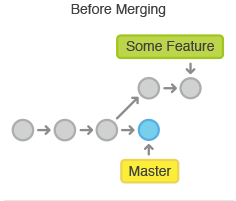
\includegraphics[scale=0.5]{3-way-merge-before}
	\end{figure}
	\begin{figure}
		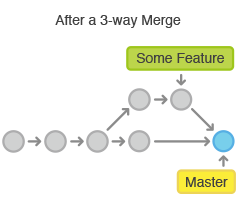
\includegraphics[scale=0.5]{3-way-merge-after}
	\end{figure}
\end{multicols}

	\begin{block}{Task: Merge the bugfix}
	Merge your bug fix to the \texttt{master} branch and then push the \texttt{master} branch. Have your colleague pull the changes before they continue working.
	\end{block}
\end{frame}
% -----------------------------------------------------------------------------


\begin{frame}[fragile]

\frametitle{Pushing a new branch to a remote}

	\begin{itemize}
	\item As with commits, newly created branches and the commits in them are (so far) stored only in the local repository
	\item  Uploading them to the remote repository is performed by pushing. 
	\item Newly created branches have to be pushed with the following command:
\begin{minted}{console}
> git push -u <remote> <branch name>
\end{minted}
	This sets up the local branch as a \textit{tracking branch} of the remote branch.
	\begin{itemize}
	\item \texttt{git status} will now show you how many new commits ahead the branches are one related to another
	\item \texttt{git push} will work without having to specify the remote
	\item When you \texttt{clone} a repository, this is automatically set up for you for the \texttt{master} branch, and for any existing branches that you check out
	\end{itemize}
	\end{itemize}
\end{frame}

% -----------------------------------------------------------------------------

\begin{frame}[fragile]

\frametitle{Pushing a new branch to a remote}

\begin{block}{Deleting remote branches}
	\begin{itemize}
	\item Can be done from the Github interface;
	\\ run \texttt{git fetch --prune} afterwards to clean them up in your local copy of the remote repository
	\item To delete a remote branch using the command-line interface, run \texttt{git push --delete <remote> <branch\_name>}
	\end{itemize}
\end{block}	

\begin{block}{Task: New feature on a remote branch}
	\begin{itemize}
	\item Create a new branch in which you will implement the feature
	\item Implement a \texttt{square} command for the demo shell program, which computes the square of the provided argument
 	\item After making the commits which implement the feature, push the feature branch to the \texttt{origin} remote.
	\end{itemize}
\end{block}	
\end{frame}

% -----------------------------------------------------------------------------

\begin{frame}[fragile]
	
\frametitle{Pull requests}

\begin{block}{Task: Pull request}
	\begin{itemize}
	\item Look for your branch in the web interface of the GitHub repository and create a pull request for the master branch of your repository. 
	\item Have your partner review the pull request. 
	\item If they find issues, correct them by pushing additional commits in the branch. The pull request will be automatically updated.
	\item Delete the branch after it has been merged.
	\end{itemize}	
	
\end{block}	

\begin{block}{Code review}

Pull requests are an efficient and transparent code review mechanism. Code review is good. Pull requests are good. Use pull requests :)
\end{block}

\end{frame}

% -----------------------------------------------------------------------------

\begin{frame}[fragile]
	
\frametitle{Working with multiple remotes}
	
\begin{block}{Why would I need multiple remotes?}
	\begin{itemize}
	\item We can get code changes from any repository, not just our remote repository (which is automatically set up as a remote named \texttt{origin} when cloning)
	\item A typical example is getting changes from the \textit{upstream} repository, i.e., the repository that we forked.
	\end{itemize}
\end{block}	

Listing and adding remotes:
\begin{minted}{console}
> git remote add <remote_name> git@<hostname>:<path to repo>	
> git remote -v	
\end{minted}
	
We can now work with the new remote in the same way as with \texttt{origin} (except we can't push into it!), e.g.:
\begin{minted}{console}
> git fetch <remote_name>
> git merge <remote_name>/<branch>
\end{minted}
	
\end{frame}

% -----------------------------------------------------------------------------

\begin{frame}

\frametitle{Merging upstream changes}

\begin{block}{Task: Merge upstream changes}
	\begin{itemize}
	\item Set up a remote called \texttt{upstream} pointing to \href{https://github.com/larics/git-tutorial-code.git}{the original repository you forked}
	\item \texttt{fetch} the \texttt{upstream} repository and compare its \texttt{master} branch with your \texttt{master} branch.
	\item Optional: for experimenting how the upstream changes will play with your changes, create a new branch.
	\item Merge the upstream \texttt{master} branch into your \texttt{master} branch (or first into your experimental branch, and then merge your experimental branch into your \texttt{master}).
	\end{itemize}
\end{block}

\end{frame}

% -----------------------------------------------------------------------------
